\chapter{Programmets brugergrænseflade}

\cbstart

I dette kapitel vil programmet grafiske brugergrænseflade blive beskrevet.


% LaTeX tabel som viser alle brugerniveauer og deres muligheder efter login.
% http://bit.ly/1kToHZ3 to edit raw table
\begin{table}
    \colorlet{shadecolor}{gray!40}
    \rowcolors{1}{white}{shadecolor}
    \begin{tabular}{l|llllll}
    ~                        & Gæst & Støttemedlem & Medlem & Elev & Underviser & Administrator \\ \hline
    Personlig forside        & ~    & ~             & \ding{51}     & \ding{51}    & \ding{51}          & \ding{51}             \\
    Se begivenheder          & \ding{51}    & \ding{51}             & \ding{51}      & \ding{51}    & \ding{51}          & \ding{51}             \\
    Tilmeld begivenheder     & ~    & ~	             & \ding{51}      & \ding{51}    & \ding{51}          & \ding{51}             \\
    Opret begivenheder       & ~    & ~             & ~      & ~    & \ding{51}          & \ding{51}             \\
    Se sejlture              & \ding{51}    & \ding{51}             & \ding{51}      & \ding{51}    & \ding{51}          & \ding{51}             \\
    Opret sejltur            & ~    & ~             & \ding{51}      & \ding{51}    & \ding{51}          & \ding{51}             \\
    Se logbøger              & \ding{51}    & \ding{51}             & \ding{51}      & \ding{51}    & \ding{51}          & \ding{51}             \\
    Opret logbog             & ~    & ~             & \ding{51}      & \ding{51}    & \ding{51}          & \ding{51}             \\
    Svar på logbog           & ~    & ~             & ~      & ~    & ~          & \ding{51}             \\
    Se undervisningstimer    & ~    & ~             & ~      & \ding{51}    & \ding{51}          & \ding{51}             \\
    Opret undervisningstimer & ~    & ~             & ~      & ~    & \ding{51}          & \ding{51}             \\
    \end{tabular}
    \caption{Tabel over alle brugerniveauer og deres tilladte funktioner.}\label{tab:permissions}\fixme{Måske skal denne tabel lige laves lidt om, enten indholdet, eller hvordan det virker i programmet.}
\end{table}

\section{Primære brugergrænseflade}
Det primære vindue tilgåes via login vinduet, som er det der starter ved programstart, eller logud. 
Der findes 4 vinduer, forskellen mellem dem er hvilke tabs der er aktive. 
I hver tab findes der en funktionalitet, samlet set findes følgende tabs:
\begin{itemize}% Denne skulle måske relatere til tabel tab:permission
    \item Forside
    \item Undervisning
    \item Begivenheder
    \item Medlemmer
    \item Både
\end{itemize}

Via hver af disse tabs, vil der være adgang til programmet forskellige funktionaliteter.
Der er også en log ud knap, som bruges til at vende tilbage til loginvinduet, således en anden bruger kan anvende systemet.
Programmet er lavet til at køre i opløsningen 1024x720 pixels.
Denne opløsning er valgt for at understøtte alt fra bærbare, med opløsninger som 1366x768 pixels i et vindue, og op til FullHD (1920x1080 pixels) osv.
Programmet har et lyst farveskema, men farverne hvid og en lys blå som hovedfarver (\#87D4EE).

\section{UserControls}
Der anvendes UserControls til at kode både brugergrænsefladen og den tilhørende code behind.


\subsection{DateTimePicker}\label{subsec:DateTimePicker}

\begin{wrapfigure}{r}{0.5\textwidth}
    \label{img:DateTimePicker}
    \vspace{-20pt}
    \begin{center}
        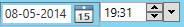
\includegraphics[width=0.48\textwidth]{Screenshots/DateTimePicker.png}
    \end{center}
    \vspace{-15pt}
    \caption{DateTimePicker}
    \vspace{-30pt}
\end{wrapfigure}

\textbf{Formål}: Denne Usercontrol, er lille i forhold til de andre der findes i programmet.
Den bruges når der skal vælges et tidspunkt som både indeholder en dato og et tidspunkt. 
Der findes en DateTimePicker i extended WPF toolkit, men da der blev opdaget en underlig fejl ved denne, blev det besluttet at en usercontrol, som gruppen selv kunne programmere, ville være bedre. 

\textbf{BrugerGrænseflade}: Den består af en DatePicker, og en TimePicker som findes i extended WPF toolkit.

\textbf{Code-Behind}: De to værdier man skriver i henholdsvis DatePickeren og TimePickeren, skal samles i en enkelt værdi som kan tilgås vha. usercontrollen. 
Dette er gjort ved at lave et property der kaldes for Value. 
Det kan ses på \myref{DateTimePickerValue} hvordan dette er blevet implementeret.
Man kan ved at assigne value igennem en instans af usercontrollen, sætte både usercontrollens TimePicker og DatePicker, og dermed give de to GUI elementer en værdi som brugerne ser.
Herudover kan man kalde dens get hvilket resultere begge værdier sat sammen, hvor TimePickeren bruger TimeOfDay, for at få et TimeSpan, som kan tilføjes direkte på den DateTime der laves fra en DatePicker, vha. + operatoren.

\begin{lstlisting}[frame=single, caption=DateTimePicker Value, label=DateTimePickerValue]
public DateTime Value
{
    get
    {
        return (DatePicker.SelectedDate.GetValueOrDefault() + TimePicker.Value.GetValueOrDefault().TimeOfDay);
    }
    set
    {
        DatePicker.SelectedDate = value;
        TimePicker.Value = value;
    }
}
\end{lstlisting}

\subsection{Forside}
\begin{figure}
    \label{img:frontpage}
    \vspace{-10pt}
    \begin{center}
        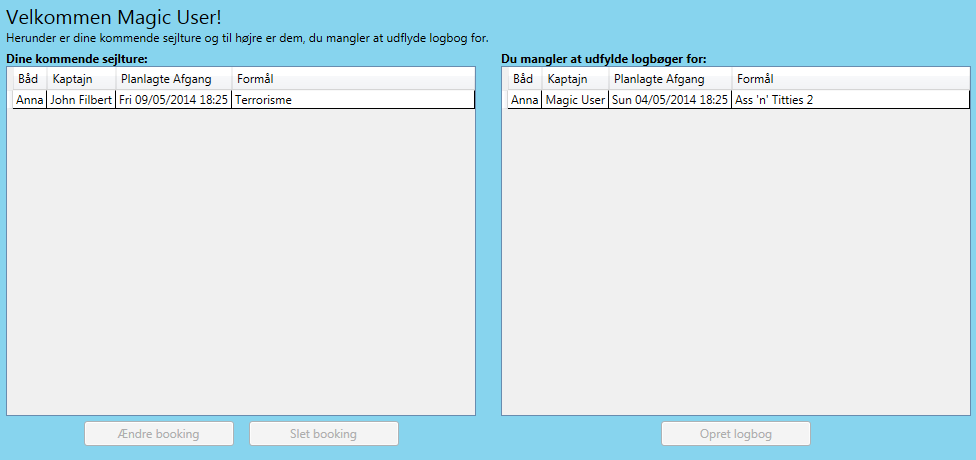
\includegraphics[scale=0.55]{UI/UserControl_FrontPage}
    \end{center}
    \vspace{-15pt}
    \caption{FrontPage-Usercontrol}
\end{figure}

\textbf{Formål}: 
Formålet med forsiden er at vise aktuel infomation på en overskulig måde for brugeren.
Det er den første side som medlemmer, og op, ser.
Fra forsiden kan man ændre og slette sine bookings, samt starte oprettelsen af en logbog.

\textbf{BrugerGrænseflade}: 
Brugergrænsefladen er forsiden består primært af to DataGrids, det venste viser de kommende sejlture og det højre viser dem personen manlger at udføre logbøger for. 
Under dem er der knapper, som bliver aktive efter en markering er udført ved, at trykke på en af rækkerne i det passende DataGrid.

\textbf{Code-Behind}: 
For at kun vise de sejlture hvor personen som er logget ind deltager i, anvendes der standard query operatorerne. 
I Listing \ref{fntpg-cb} er et udsnit af koden, nærmere bestemt den del som vælger de rigtige sejlture.
Det første udtryk finder de ture som er i fremtiden, hvor personen indgår i besætningslisten, ud fra alle turene.

Det andet udtryk finder de ture, hvor den nuværende person er kaptajn for, som er forventet at være returneret til havn og ikke har nogen logbog. 

Begge udtryk returnerer en IEnumerable som derefter assignes som DataGridenes ItemSource.

\begin{lstlisting}[frame=single, caption=Forsidens Code-Behind, label=fntpg-cb]
UpcommingTripsDataGrid.ItemsSource =
    sailTripList.Where(t => t.Crew.Select(p => p.PersonId).Contains(usrId))
        .Where(t => t.DepartureTime > DateTime.Now);

LogbookDataGrid.ItemsSource =
    sailTripList.Where(t => t.Captain.PersonId == usrId && t.ArrivalTime < DateTime.Now && t.Logbook == null);
\end{lstlisting}

\subsection{Boat user control}

\begin{wrapfigure}{l}{0.5\textwidth}
    \label{img:boat_scr}
    \vspace{-20pt}
    \begin{center}
        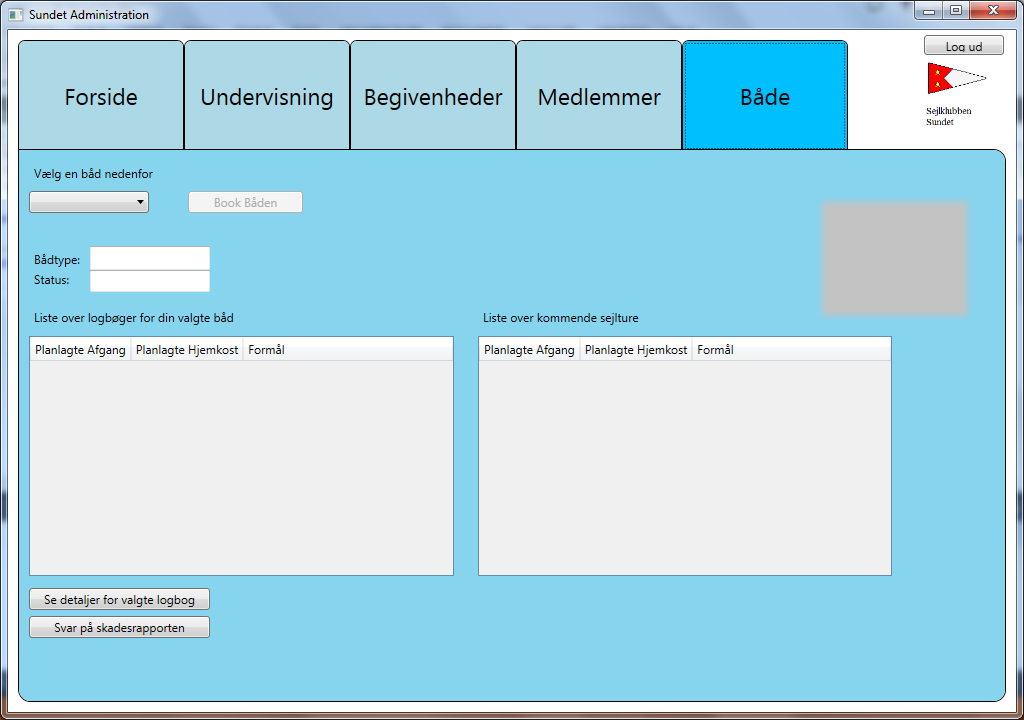
\includegraphics[width=0.48\textwidth]{/Screenshots/boat_scr.png}
    \end{center}
    \vspace{-20pt}
    \caption{Boat screenshot}
    \vspace{-10pt}
\end{wrapfigure}

\textbf{Formål:}

Under Boat kan man få et overblik over hvilke både som der er til rådighed i sejlklubben inklusiv bådtype og status på båden (om den f.eks. er operationel). 
Man kan også booke en båd, se liste over logbøger for en valgt båd og ligeledes se en liste over kommende sejlture (bookings). 

\textbf{Brugergrænseflade:}

På siden findes der flere forskellige controls.
Man starter først med en dropdown menu, hvor man kan vælge hvilken båd man vil se informationer om.
Til højre for den er der en knap ``Book Båden'', som man kan trykke på, hvis man vil booke båden. Når den trykkes på, så åbner der en ny fane, hvor man kan angive bookingsinformation. 
Helt ude til højre er der et billede af hver enkelt båd. 
Under dropdown menuen bliver der vist i en textbox bådtypen og bådens status. 
Til visning af logbøger og kommende sejlture, er der to listbokse ved siden af hinanden, hvor hhv. logbøger og kommende sejlture vises efter dato. 
I selve listboksene kan man se ``Planlagte afgang'', ``Planlagte hjemkomst'' og ``Formål'', ved både logbøger og kommende sejlture. 
Til sidst er der to knapper; ``Se detaljer for valgte logbøger'' og, hvis man er logget ind som administrator, ``Svar på skadesrapporten''. Ved at først vælge en logbog, i listen over logbøger, og derefter klikke på ``Se detaljer for valgte logbøger'', så kan man se detaljer omkring den valgte logbog. 
Hvis der dobbeltklikkes på en logbog i listboksen, så opnår man samme effekt. 
Hvis man er logget ind som administrator, så man kan vælge en logbog, og trykke på ``Svar på skadesrapporten'', hvor der åbnes et nyt vindue, hvor der kan svares på skadesrapporten. 

\textbf{Code-behind:}

Metoden BoatComboBox\_OnSelectionChanged aktiveres ved at vælge en båd i dropdown menuen. 
Hvis der ikke er valgt en båd, så er Book Button (``Booking'') ikke aktiv. 

Først noget hentning af data fra dal og sortering\fxnote{Skal skrives når database oprettes}

Efter dataet er hentet fra \textbf{databasen}, så tjekkes der, at hvis brugeren ikke er supportmedlem, så er BookButton (``Booking'') aktiv. 

Derefter laves der et tjek på om ImagePath er null, hvis ikke, så er billedestien ImagePath, så hver båd har sit eget billede. 
Hvis ImagePath er null, så bliver der vist et gråt billede.

Derefter tjekkes der om båden er operationel og bådtypen hentes og vises i hver deres textbox. 

Til sidst så bliver dataet som hentes fra \textbf{databasen} afbildet i hvert sit datagrid.\fxnote{sæt kode ind}


\section{Vinduer}


\subsection{Login brugergrænseflade}
\begin{wrapfigure}{r}{0.5\textwidth}
    \label{img:login_interface}
    \vspace{-20pt}
    \begin{center}
        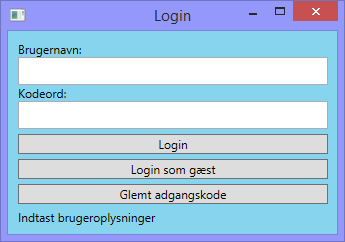
\includegraphics[width=0.48\textwidth]{UI/Login_Window_Empty_Fields.png}
    \end{center}
    \vspace{-15pt}
    \caption{Login interface}
\end{wrapfigure}
 
\textbf{Formål}: 
Login brugergrænsefladen har til formål at verificere en brugers identitet. 
Det er det første vindue brugeren ser, og åbner hovedvinduet.
 
\textbf{BrugerGrænseflade}: 
Brugergrænsefladen til loginvinduet er meget simpel og lige til. 
Der er en TextBox til brugernavnet og en PasswordBox til kodeordet.
En PasswordBox er en TextBox hvor de intastede karakterer vises som en sort prik, i stedet for de skrevne tegn, for at beskytte brugeren.
Login knappen trykkes efter brugeren har indtastet sine brugeroplysninger, den åbner hovedvinduet hvis infomationen er korrekt.
``Login som gæst''-knappen kræver ingen brugeroplysninger og åbner en let udgave af hovedvinduet, uden særlige tilladelser.
Til sidst er en TextBlock som giver brugen indikationer hvis der er skrevet forkert.
 
\textbf{Code-Behind}: 
Den centrale del af det Code-Behind som er i forbindelse med loginvinduet, er der der verificerer at en bruger findes og koden er korrekt.
I \myref{dologin} vises det stykke kode som tjekker brugeroplysningerne.
Først sikres det er der findes medlemmer i databasen af sejlklubmedlemmer.
Herefter hentes den anmodede bruger, udtrykket sammenligner det indtastede brugernavn, med alle dem i databasen, dette er case insensitive (Altså vil ``FoOBar'' være lig med ``foobar'' og ``FOOBAR'').
Hvis brugen findes så sammenlignes det indtastede kodeord med det i databasen, her anvendes en hashing algoritme. 
Den sikrer at hvis noget får adgang til databasen, kan de ikke se brugernes kodeord.
Er alt infomation gyldigt så kaldes ``LoginCompleted''-metoden med argumentet ``usr'' som er brugeren. 
 
\begin{lstlisting}[frame=single, caption=DoLogin, label=dologin]
private void DoLogin(object sender, RoutedEventArgs e)
{
    // If usernamebox or password is empty display an error message.
    [...]
 
    if (sailClubMembers != null)
    {
        SailClubMember usr =
            sailClubMembers.FirstOrDefault(
                x => String.Equals(x.Username, UsernameBox.Text, StringComparison.CurrentCultureIgnoreCase));
 
        // Check if user exists (Case insensitive)
        if (usr != null &&
            String.Equals(usr.Username, UsernameBox.Text, StringComparison.CurrentCultureIgnoreCase))
        {
            // Check if the password is correct (Case sensitive)
            if (usr.PasswordHash == EncryptionHelper.Sha256(PasswordBox.Password))
            {
                LoginCompleted(usr);
            } 
 
            // Code to show errors for wrong infomation
            [...]
        }
    }
}
\end{lstlisting}


\subsection{CreateBoatBookingWindow}

\begin{wrapfigure}{R}{0.5\textwidth}
    \label{img:boatBookWindow}
    \vspace{-20pt}
    \begin{center}
        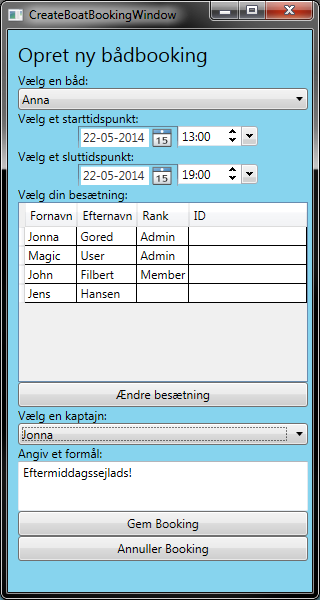
\includegraphics[width=0.48\textwidth]{UI/CreateBoatbookingWindow.png}
    \end{center}
    \vspace{-20pt}
    \caption{CreateBoatbookingWindow}
    \vspace{-30pt}
\end{wrapfigure}

\textbf{Formål}: 
Dette vindue opretter, eller ændrer, en \textbf{RegularTrip} (En bådbooking).
Dette vindue anvendes fire stedder i programmet, fra \textbf{Boats}-UserControllen, \textbf{NewLecture}-vinduet (under Undervisning), og fra \textbf{FrontPage}-UserControllen eller \textbf{Boats}-UserControllen (Til at redigere en booking). 

\textbf{BrugerGrænseflade}: 
Vinduet er opbygget af et vertikalt StackPanel.
Først vælges en båd, her anvendes en ComboBox da der skal vælges en værdi fra en liste.
Herefter anvendes \textbf{DateTimePicker}-UserControllen til at vælge et start- og sluttidspunkt.
Der vises den nuværende besætning, samt muligheden for at ændre den ved at trykke på en Button med labellet ``Ændre Besætning''.
Når en besætning er valgt, kan der vælges en kaptajn ud fra besætningslisten.
Tilsidst er der en TextBox, hvori brugeren kan angive formålet med turen.
Derudover er der to Buttons, en til at gemme og en til at annulere.

\textbf{Code-Behind}: 
Til vinduet er der tre constructors, dette er således de fire stedder hvorfra vinduet åbnes, hver kan behande det på deres måde, da to af dem er ens. 
De tre constuctors er i Listing \ref{threeConstructors}.
Den første constuctor skaber et nyt vindue, herunder henter den bådede fra DataBasen og bliver kaldt fra Boats-UserControllen.
Den vælger også den båd, som er angivet i dens index parameter.
De to DateTimerPickere sættes også til det nuværende tidspunkt, dette gør det nemmere at vælge et passende tidspunkt for den kommende booking.

De to andre constructors kalder, den første da den er grundlæggende for at kunne bruge vinduet. 
Constructoren med forskiften ``CreateBoatBookingWindow(RegularTrip rt) : this(-1)'', ændrer teksten på gem knappen fra ``Gem Booking'' til ``Ændre Booking''. \fixme{Skal der være nutids-r på ændre(r)?}
Samt den ændre hvilken methode den kalder, således der ikke forsøges at oprette en ny sejltur, men derimod opdateres en ekstisterende. 
Fælles for de to metoder som kaldes af knappen er at de skal verificere gyldigheden af en tur. 
Dette udføres i ``CreateSailTrip()'' som returner en gyldig instans af SailTrip-klassen hvis turen er gyldig, eller null og en fejlbesked hvis den ikke er. 
Dette null bliver håndtereret af kaldermetoden, således der ikke opstår exceptions.

\begin{lstlisting}[frame=single, caption=De tre constuctoreres forskrifter, label=threeConstructors]
// Called to Initialize the window, from the other constructors and from the Boats-UserControl
public CreateBoatBookingWindow(int index)
{
    InitializeComponent();

    // Initialize ComboBoxes and Databaseforbindelsen
    [...]

    // Set DateTimerPickers to the current time.
    [...]
}

// Called to edit a trip from the FrontPage
public CreateBoatBookingWindow(RegularTrip rt) : this(-1)
{
    // Sets all the value from the input RegularTrip
    [...]

    // Change the text and behaveour of the buttons
    [...]
}

// Called from NewLecture
public CreateBoatBookingWindow(DateTime departure, DateTime arrival, Team currentTeam) : this(-1)
{
    // Sets values to match the parameters given
    [...]

    // Set the Captain to be the tracher
    [...]

    // Add a description of the class in the PurposeTextBox.
    [...]

    // Call the SaveFunction
    [...]
}
\end{lstlisting}

\subsection{CreateCrewWindow}

\begin{wrapfigure}{r}{0.5\textwidth}
    \label{img:login_interface}
    \vspace{-20pt}
    \begin{center}
        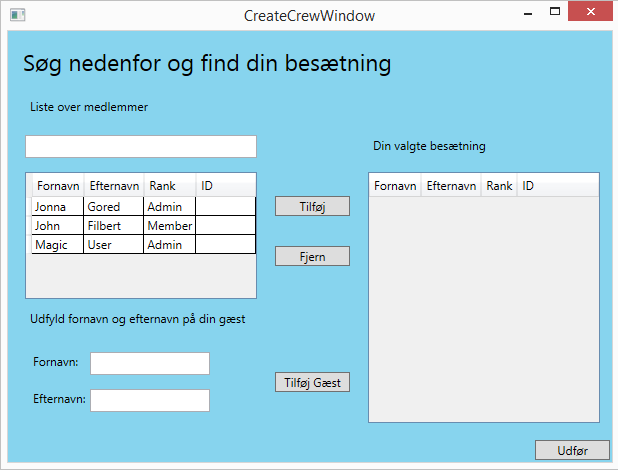
\includegraphics[width=0.48\textwidth]{Screenshots/CreateCrewWindow.png}
    \end{center}
    \vspace{-20pt}
    \caption{CreateCrewWindow}
    \vspace{-30pt}
\end{wrapfigure}

\textbf{Formål}: Dette vindue åbnes op to steder i programmet: \textbf{CreateLogbookWindow} og i \textbf{CreateBoatBookingWindow}. Det bruges når der skal laves en besætning til en RegularSailtrip.  

\textbf{BrugerGrænseflade}: Der er to datagrids som indeholder to lister. Listen til venstre består af SailClubMembers som bliver hentet ind fra databasen. Listen til højre indeholder det Crew som man er i gang med at udforme til enten RegularSailTrip, eller Logbook. Der er også tilføjet tekstfelter, så man kan skrive navnet på en gæst man tog med på sejlturen. Der er knapper som tilføjer de forskellige personer til Crewlisten. Øverst findes også et tekstfelt til at søge listen over medlemmer igennem. Når man har lavet sin liste, kan man trykke udfør, for at komme tilbage til vinduet der kaldte CreateCrewWindow.

\textbf{Code-Behind}: 
På \myref{AddGuestButton} kan man se koden der sker når man trykker på knappen med teksten Tilføj Gæst.
Der er blevet brugt et \textbf{regular expression} til at tjekke om den string brugeren angiver i de to tekstbokse for gæstens navne er lovlige. 
Det er blevet valgt man må bruge hele det danske alfabet samt mellemrum, så navne såsom: Lars Peter Vesterager, er mulige.
Hvis begge tekstbokse er lovlige, kommer man ind i det inderste if-statement, hvor der laves en ny person med det pågældende FirstName og LastName. 
Derefter tilføjes personen til Listen der vises i Datagridded til højre, og til sidst kaldes RefreshDatagrid, som man kan se på \myref{RefreshDatagrid}.

\begin{lstlisting}[frame=single, caption=Add Guest Buttton, label=AddGuestButton]
{
    if (Regex.IsMatch(FirstNameBox.Text, "^[A-ZÆØÅa-zæøå ]*$") && FirstNameBox.Text.Trim() != String.Empty)
    {
        if (Regex.IsMatch(LastNameBox.Text, "^[A-ZÆØÅa-zæøå ]*$") && LastNameBox.Text.Trim() != String.Empty)
        {
            var p = new Person();
            p.FirstName = FirstNameBox.Text;
            p.LastName = LastNameBox.Text;
            CrewList.Add(p);

            RefreshDatagrid(CurrentCrewDataGrid, CrewList);

            FirstNameBox.Clear();
            LastNameBox.Clear();
        }
    }
    else
    {
        MessageBox.Show("Ugyldigt navn. \nPrøv venligst igen");
    }
}      
\end{lstlisting}

Her modtages der et Datagrid, som skal have dets Itemssource Refreshet, og en ICollection, som er det data der skal sættes ind i Datagridded. 
Det gøres ved at assigne dets Itemssource til null, og derefter assigne det tilbage til den ICollection der blev sendt med. 

\begin{lstlisting}[frame=single, caption=Refresh Datagrid, label=RefreshDatagrid]
private void RefreshDatagrid(DataGrid Grid, ICollection<Person> list)
{
    Grid.ItemsSource = null;
    Grid.ItemsSource = list;
}
\end{lstlisting}

Knappen til at tilføje et medlem kan ses på \myref{AddMember}.
Inden det valgte medlem tilføjes til listen tjekkes der om medlemmet allerede findes i den anden liste. 
Dette gøres ved at anvende standard query operatorerne. 
Først et where med et lambda udtryk hvor der findes alle SailClubMembers i listen. 
Herefter castes disse om til SailClubMembers, for derefter at kunne tjekke om det valgte medlems SailClubMemberId er forskelligt fra de andre i listen. 
Hvis det hele er true, så bliver det valgte medlem tilføjet til listen, og RefreshDataGrid kaldes for at opdatere Datagridded.

\begin{lstlisting}[frame=single, caption=Add Member, label=AddMember]
private void AddButton_OnClick(object sender, RoutedEventArgs e)
{
    var currentPerson = (SailClubMember) MemberDataGrid.SelectedItem;

    if (
        CrewList.Where(x => x is SailClubMember)
            .Cast<SailClubMember>()
            .All(x => x.SailClubMemberId != currentPerson.SailClubMemberId))
        CrewList.Add(currentPerson);

    DataGridCollection.Filter = Filter; 
    RefreshDatagrid(CurrentCrewDataGrid, CrewList);
}
\end{lstlisting}

\subsection{CreateLogbookWindow}

\begin{wrapfigure}{r}{0.5\textwidth}
    \label{img:login_interface}
    \vspace{-20pt}
    \begin{center}
        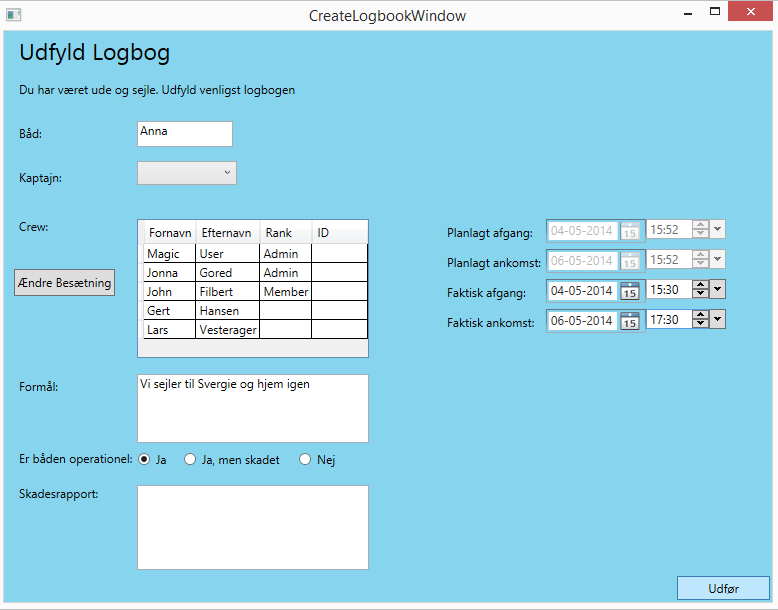
\includegraphics[width=0.48\textwidth]{Screenshots/CreateLogbook.png}
    \end{center}
    \vspace{-15pt}
    \caption{CreateLogBookWindow}
    \vspace{-30pt}
\end{wrapfigure}

\textbf{Formål}: Dette vindue bruges når et medlem som har booket en båd, skal udfylde sejlturens logbog. Vinduet tilgås fra usercontrollen FrontPage. Medlemmet skal udfylde de forskellige felter der findes i vinduet og trykke udfør, for at gemme logbogen i databasen.

\textbf{BrugerGrænseflade}: Der er mange elementer på dette skærmbillede. Øverst til venstre finder man en textbox, som udfyldes automatisk når man vil udfylde sin logbog. 
Textboxen indeholder navnet på den båd, logbogen skrives for, og dette loades igennem den RegularSailtrip, som logbogen skrives for.
Under den findes en combobox hvor man vælger Kaptajn eller bådføren for sejlturen.
Her kan vælges imellem alle de personer som er sat på besætningslisten. 
Der bliver altså ikke tjekket om personerne har duelighedsbevis, da gæsterne netop også kan være kaptajnen eller bådføren.
Under dette finder man en boks hvor man angiver turens formål. 
Der er desuden tre RadioButtons, som angiver hvilken tilstand båden er i. 
Hvis man aktivere enten knappen med teksten: "Ja men skadet" eller "nej", så påkræves det at man udfylder dette felt. 

Til højre finder man 4 DateTimePicker usercontrols, som beskrevet i \myref{subsec:DateTimePicker}. De to øverste er ikke enabled, da de også er loaded fra den RegularSailtrip man udfylder logbog for. De to andre skal dog udfyldes, og ændres fra de standardværdier som de har når man åbner vinduet. 

Under disse DateTimePickers, finder man endnu en textbox, som skal udfyldes med en vejrrapport.

Der findes et lignende vindue som hedder ViewSpecificLogbookWindow.
Dette vindue indeholder alle de samme felter, men har også et svar fra BoatChief som findes i en textbox.
Alle elementerne i det vindue er sat til Readonly eller IsEnabled="False", da man kun skal kunne se logbogen i det vindue, og altså ikke udfylde noget.


\textbf{Code-Behind}: Der er ikke meget kode at se på ved dette vindue, da meget af det er simpelt, men man kan se på den kode der findes bag knappen med teksten: "Udfør".
Koden for dette kan ses på \myref{SaveLogbookButton}.
Først tjekkes der om de forskellige felter i vinduet er udfyldt, og hvis alt er udfyldt kommer man ind i det sidste else if-statement der ses i koden. 
Her afsættes der om båden har taget skade under sejlturen, og derefter gemmes alle felterne i de lokale kopier af både RegularSailTrip og Logbook, hvor der til slut kaldes updateDatabase på de to lokale objekter.

\begin{lstlisting}[frame=single, caption= Gem Logbog, label=SaveLogbookButton]
private void FileLogbookButton_OnClick(object sender, RoutedEventArgs e)
{
	if (YesRadioButton.IsChecked == false && NoRadioButton.IsChecked == false)
	{
	    MessageBox.Show("Udfyld venligst om båden blev skadet under sejladsen");
	}
	...
	else if (YesRadioButton.IsChecked == true || NoRadioButton.IsChecked == true
	            || YesButBrokenRadioButton.IsChecked == true) 
	{
	        if (YesRadioButton.IsChecked == true)
	        {
	            currentLogbook.DamageInflicted = false;
	        }      
	        if (NoRadioButton.IsChecked == true || YesButBrokenRadioButton.IsChecked == true)
	        {
	            currentLogbook.DamageInflicted = true;
	        }
	    RegularSailTrip.PurposeAndArea = PurposeTextBox.Text;
	    currentLogbook.DamageDescription = DamageTextBox.Text;
	    currentLogbook.ActualCrew = CrewList;
	    currentLogbook.ActualArrivalTime = DateTimePickerActualArrival.Value;
	    currentLogbook.ActualDepartureTime = DateTimePickerActualDeparture.Value;
	    currentLogbook.FiledBy = _currentSailClubMember;
	    RegularSailTrip.WeatherConditions = WeatherConditionTextBox.Text;
	    RegularSailTrip.Crew = CrewList;
	    RegularSailTrip.Logbook = currentLogbook;
}
\end{lstlisting}

\fxnote{Opdater denne listning med Update Database kaldet.}


\subsection{Undervisning}
Undervisnings delen i programmet består af to 'Usercontrols' og to 'Windows'.
Af 'Usercontrols' eksistere 'StudyTeacher' som er det et medlem med undervisning eller admin status kan se.
Den anden 'Usercontrol' er 'StudyStudent' hvilket er den studenter har adgang til, hvis man hverken er student, underviser eller admin har man således ikke adgang til nogle af disse. 
'StudyStudent' er programmeringsmæssigt meget begrænset i det dens eneste funktion er at repræsentere den enkelte students information, hvilket kun er tilgængelig for student på et read-only niveau.
I 'StudyTeacher' delen kan en underviser oprette lektioner og hold, slette hold, ændre på hold samt fuldføre uddannelsesforløbet ved at angive studenter deres duelighedsbevis.

\subsubsection{Brugergrænsefladen}
\paragraph*{StudyTeacher}
\begin{figure}[htbp]
  \centering
  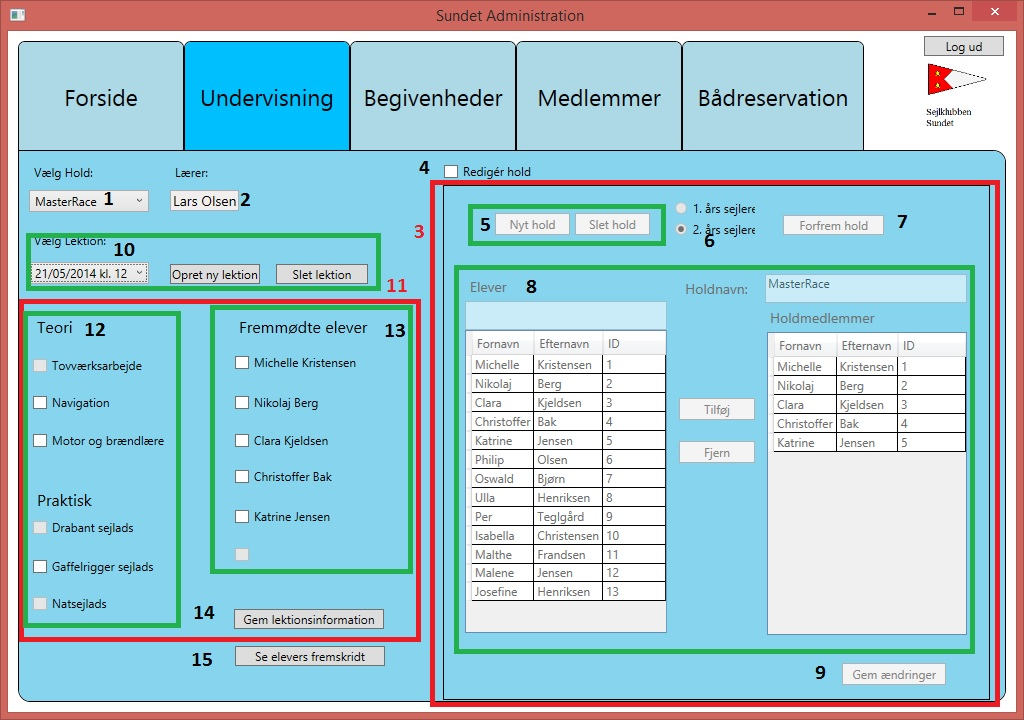
\includegraphics[width=1\textwidth]{images/UI/StudyTeacherMarked.jpg}
  \caption[UIStudyTeacher]{UI for undervisning tab som underviser og admin, markeringer bruges til forklaringer nedenfor}
  \label{fig:StudyTeacher}
\end{figure}

På \myref{fig:StudyTeacher} ses en 'Usercontrol' for 'StudyTeacher' på de markerede områder ses grupperinger af brugergrænsefladens funktioner som er sammenhængende.
\textbf{1} Referere til en 'ComboBox' som benyttes til valg af hold. 
Denne 'ComboBox' har indflydelse på det meste af undervisningsdelen, da denne information er afhængig af hvilket hold, som er valgt.
\textbf{2} Henviser til en 'CheckBox', som har kontrol over \textbf{3}, et 'Grid' indeholdende funktionalitet til brug af redigering samt kreation af hold.
\textbf{4} er tilføjning og sletning af hold, slet hold knappen sletter det hold som er valgt i \textbf{1}, mens nyt hold knappen åbner et 'nested window', 'NewTeam', i programmet hvor et nyt hold kan blive oprettet.
\textbf{5} Disse 'Radio Buttons' benyttes for at vælge om holdet er 1. års eller 2. års sejlere.
\textbf{6} Dette område benyttes til at tilføje medlemmer til et hold, at fjerne dem igen ved brug af tilføj og fjern knapperne. 
Det venstre 'DataGrid' benyttes til søgning af medlemmer, i dette grid kan findes alle 'StudentMember', mens i det højre 'DataGrid' ses de studerende som der på det valgte hold i \textbf{1}.
\textbf{7} Denne knap gemmer ændringer for holdet, dette er lavet separat for at undgå kommunikation med database ved hvert klik.
\textbf{8} Denne knap forsøger at angive et duelighedsbevis til de medlemmer på det valgte hold i \textbf{1} som opfylder alle undervisningskrav.
\textbf{9} Referer til et grid med lektionsinformation, hvis der ikke er valgt en lektion i \textbf{13} er dette 'Grid' ikke muligt at benytte.
\textbf{10} Denne række af 'CheckBoxe' bruges til at krydse af hvad der er blevet undervist i på den valgte lektion, \textbf{11} benyttes ligeledes til at afkrydse hvilke elever var til stede.
\textbf{12} Fungerer for lektion ligesom \textbf{7} for hold og er lavet for samme formål.
\textbf{13} Er en 'ComboBox' som bruges til valg af lektion.
Den sidste funktion \textbf{14} åbner et nyt 'Window', 'NewLecture', hvor man kan oprette en ny lektion for det givne hold valgt i \textbf{1}.

\paragraph{StudyStudent}

\begin{figure}[htbp]
  \centering
  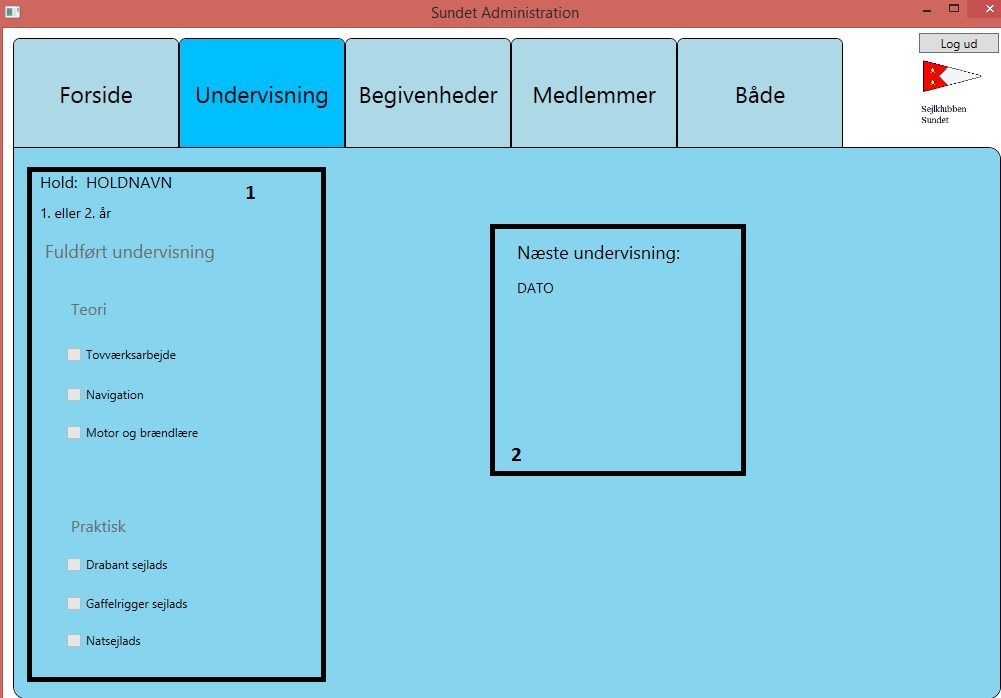
\includegraphics[width=1\textwidth]{images/UI/StudyStudentMarked.jpg}
  \caption[UIStudyStudent]{UI for undervisning tab som student, markeringer bruges til forklaringer nedenfor}
  \label{fig:StudyStudent}
\end{figure}

På \myref{fig:StudyStudent} ses en 'Usercontrol' for 'StudyStudent'. \textbf{1} Indeholder information omkring personens undervisning, 'CheckBox'ene' indikere undervisningsområder for den student som er logget ind, mens texten ovenfor viser hvilket hold personen er på. \textbf{2} Viser den næste lektionstidspunkt for det hold studenten er tilknyttet.

\paragraph{NewLecture og NewTeam}

\begin{figure}[htbp]
\centering
\begin{minipage}{.5\textwidth}
  \centering
  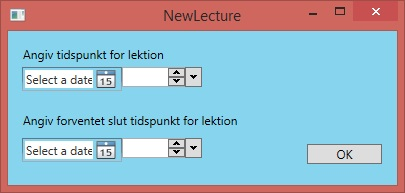
\includegraphics[width=0.8\textwidth]{images/UI/NewLecture.jpg}
  \caption[UINewLecture]{UI for NewLecture window}
  \label{fig:NewLecture}
\end{minipage}%
\begin{minipage}{.5\textwidth}
  \centering
  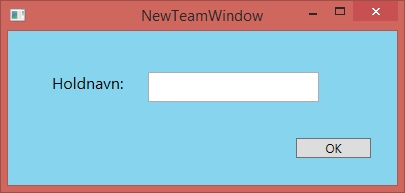
\includegraphics[width=0.8\textwidth]{images/UI/NewTeam.jpg}
  \caption[UINewTeam]{UI for NewTeam window}
  \label{fig:NewTeam}
\end{minipage}%
\end{figure}

På \myref{fig:NewLecture} ses et 'Window' for 'NewLecture'. 
I 'NewLecture' vælges der to datoer ud i fremtiden, disse bruges til at oprette en lektion, dette sker når der trykkes 'OK'. 
På \myref{fig:NewTeam} ses 'NewTeam', her skrives et holdnavn i tekstboksen, og således kan et hold oprettes.

\subsubsection{Code-Behind}
\paragraph{StudyTeacher}
\paragraph{StudyStudent}
\paragraph{NewLecture}
'NewLecture' er for brugeren simpel at benytte, der er dog mere funktionalitet i dette vindue end der bliver vist for brugeren.

\begin{lstlisting}[caption={Kode for 'OK' knap i 'NewLecture' 'Window'.}\label{NewLectOk}]
private void CompleteLectureCreate_Click(object sender, RoutedEventArgs e)
        {
            var lecture = new Lecture
            {
                DateOfLecture = DateTimePickerPlannedLectureTime.Value
            };
            DalLocator.LectureDal.Create(lecture);
            var Departure = DateTimePickerPlannedLectureTime.Value;
            var Arrival = DateTimePickerPlannedLectureTimeEnd.Value;
            var book = new CreateBoatBookingWindow(Departure, Arrival, _currentTeam);
        }
\end{lstlisting}
I \myref{NewLectOk} ses koden for at trykke på OK knappen i 'NewLecture' vinduet. DateTimePicker bliver aflæst og informationen brugt til at oprette en 'Lecture', yderligere bliver informationen også gemt i henholdsvis 'Departure' og 'Arrival'. Disse bliver således videresendt i en constructer for booking af både, 'CreateBoatBookingWindow()'. Dette er OK knappens indirekte funktionalitet, funktionaliteten af dette kan ses på \myref{IndirekteBook}.

\begin{lstlisting}[caption={Dette kode bliver indirekte udført når der trykkes på 'OK' knappen, og opretter en bådreservation for lektionen.}\label{IndirekteBook}]
public CreateBoatBookingWindow(DateTime departure, DateTime arrival, Team currentTeam) 
	   : this(-1)
        {
            List<Boat> boats = new List<Boat>();
            boats = DalLocator.BoatDal.GetAll().ToList();
            Boat Anya = new Boat
            {
                Type = (currentTeam.Level == Team.ClassLevel.Second) ? BoatType.Gaffelrigger 
                : BoatType.Drabant
            };

            Boat currentBoat = boats.FirstOrDefault(
                x => x.Type == Anya.Type);

            BoatComboBox.SelectedIndex = boats.FindIndex(b => b == currentBoat);
            CrewList.Add(GlobalInformation.CurrentUser);
            CaptainComboBox.SelectedIndex = 0;
            foreach (var member in currentTeam.TeamMembers)
            {
                CrewList.Add(member);
            }
            DateTimeStart.Value = departure;
            DateTimeEnd.Value = arrival;
            PurposeTextBox.Text = "Undervisning af:" + currentTeam.Name;
            SaveButton_Click(new object(), new RoutedEventArgs());
        }
\end{lstlisting}
Denne constructer nedarver fra 'CreateBoatBookingWindow()' constructeren som kun tager en paramter, index, hertil benyttes ': this(-1)', ses på linje 2, for at sætte ComboBox'en, der styrer valg af booking, kan ses på <indsæt reference til BoatBooking>\fxnote{look at <>}, til null.
Alt efter om sejler holdet er et 1. eller 2. års sejlerhold, skal der bookes henholdsvis en drabant eller en gaffelrigger, dette håndteres på linje 6 - 15. Der laves en lokal båd, Anya, hvis 'BoatType' bliver sat gennem en 'conditional operator'.
Herefter benyttes et 'lambda expression' til at finde den første båd af den korrekte type i databasen og 'BoatComboBox', som styrer valg af båd, bliver sat til denne.
Efterfølgende bliver den admin eller underviser der opretter lektionen sat som kaptajn, det medsendte hold tilføjes 'CrewList', Departure og Arrival sættes også til de medsendte værdier, Formål bliver sat til undervisning og til sidst kaldes det event som fuldfører bookningen.

\cbend
